\newchapter{c:ctfPFF}{Design of the PFF Prototype at CTF3}

This is the introductory text.

\newsection{s:ctfIntro}{CTF3}

\subsection{Goals of CTF3}
\label{ss:ctfGoals}

CLIC and PFF

\subsection{Layout of CTF3}
\label{ss:ctfLayout}

\begin{figure}
  \centering
  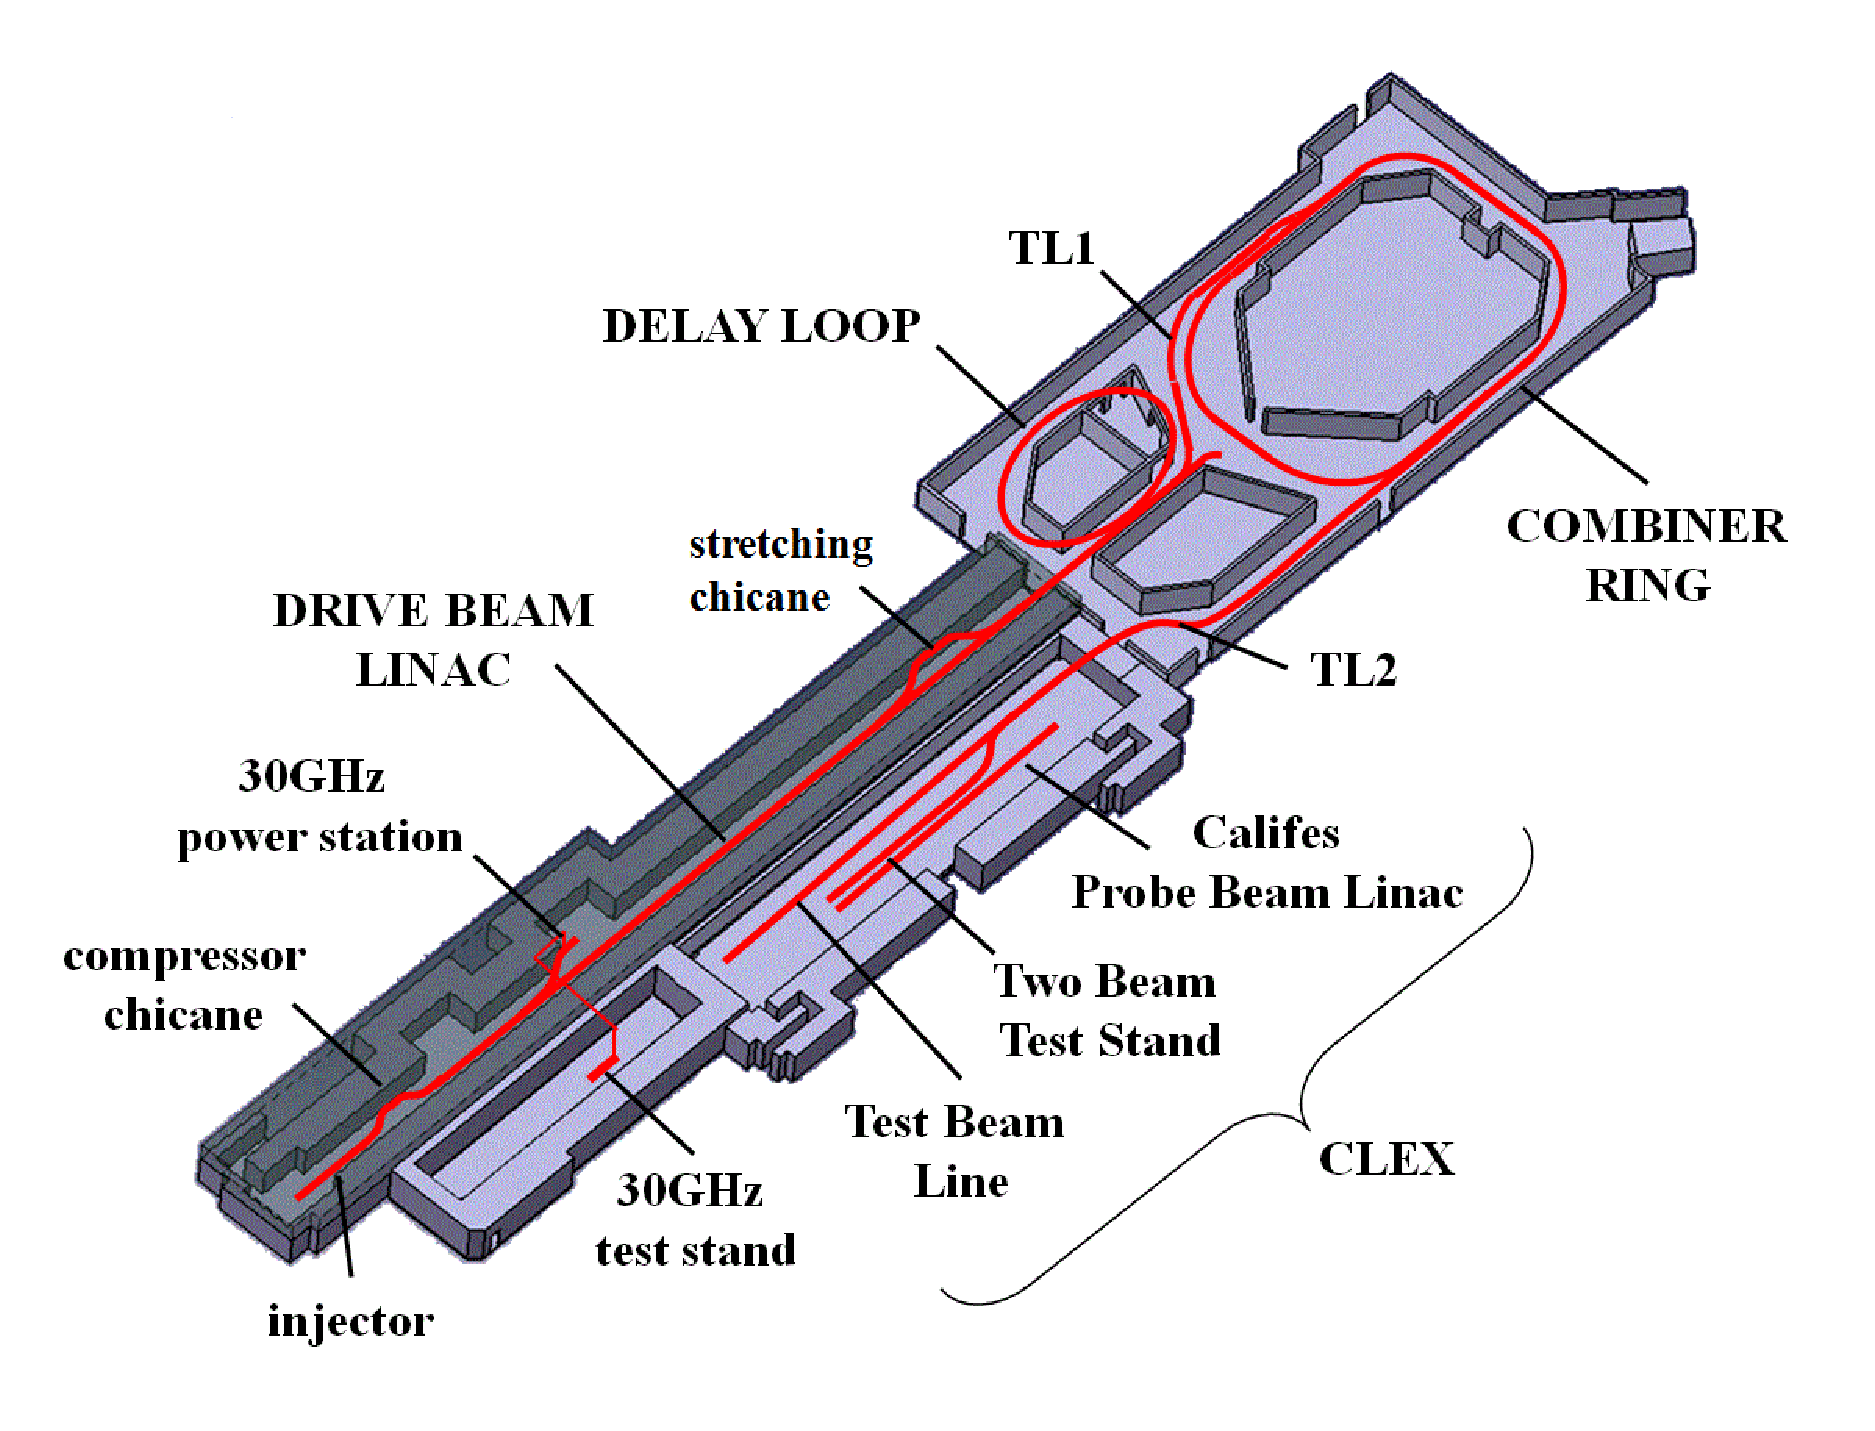
\includegraphics[width=0.45\textwidth]{Figures/ctfLayout}
  \caption{CTF3 schematic.}
  \label{f:ctfLayout}
\end{figure}

\newsection{s:pffCTFIntro}{Design of the PFF Prototype at CTF3}

\subsection{Schematic Overview of PFF System}
\label{ss:ctfPFFLayout};

\subsection{Latency}
\label{ss:availLatency};

\newsection{s:pffHardware}{PFF Hardware}

\subsection{FONT5 Board}
\label{ss:font5}

\subsection{Amplifier}
\label{ss:amplifier}

\subsection{Phase Monitors}
\label{ss:phMons}

\subsection{Kickers}
\label{ss:kickers}

\newsection{s:ctfVsCLIC}{Differences Between PFF at CTF and CLIC}

\subsection{Phase Sag}
\label{ss:phaseSag}

\subsection{Pulse Length}
\label{ss:pulseLength}

\newsection{s:pffEquations}{Feedforward Algorithm}

\subsection{Theoretical Corrected Jitter}
\label{ss:theoryJitter}

\subsection{Theoretical Optimal Gain}
\label{ss:theoryGain}


